%\documentclass[preprint, review, 3p, authoryear]{elsarticle}
\documentclass[10pt, a4paper]{article}

%\usepackage{setspace}
\usepackage[utf8]{inputenc}
\usepackage{amsmath, amssymb, amsthm, bbm}
\usepackage{xcolor}
\usepackage{graphicx}
\usepackage[authoryear]{natbib}
\usepackage{apalike}
\usepackage{relsize}
\usepackage{array}
\usepackage{multirow}
\usepackage{showlabels}
\usepackage{setspace}
\usepackage[normalem]{ulem}
\usepackage{xspace}
%Add line numbering
%Line numbering can be incorporated by using the lineno package. Add these statements in the preamble:
\usepackage{lineno}
\linenumbers

\DeclareMathOperator*{\argmax}{arg\,max}

\newtheorem{prob}{Problem}
\newtheorem{prop}{Proposition}
\newtheorem{definition}{Definition}

%%%%% bold symbol in math enviornment
\newcommand{\m}[1]{\boldsymbol{#1}}

\newcommand{\fmm}{\textsc{fmm}\xspace}

\title{Merging the components of a finite mixture using  posterior probabilities}
\author{M. Comas-Cufí \and J.A. Martín-Fernández \and G. Mateu-Figueras}

%\doublespacing
\begin{document}

\begin{spacing}{1.9}

\pagenumbering{arabic}

\maketitle

\section{Introduction}

%Cl
The most standard parametric approach in cluster analysis assumes data can be modelled by a \emph{finite mixture of distributions} or a \emph{finite mixture model} (\fmm). A \fmm is a probability distribution with probability density function (pdf) defined as the linear combination of pdf from distributions with domain $\mathbb{X}$. In general, the pdf $f$ of a \fmm is
\begin{equation}\label{mixt}
f(\;\cdot\; ; \pi_1, \dots, \pi_k, \m\theta_1, \dots, \m\theta_k) = \pi_1 f_1(\;\cdot\; ; \m\theta_1) + \dots + \pi_k f_k(\;\cdot\; ; \m\theta_k),
\end{equation}
where $\m\theta_1, \dots,  \m\theta_k$ are the parameters of the pdf $f_1, \dots, f_k$ respectively and, because $\int_{\mathbb{X}}f = 1$ the restriction $\sum_{\ell = 1}^k \pi_\ell = 1$ holds. The pdf $f_1, \dots, f_k$ are called the \emph{components} of the \fmm, or simply the \emph{mixture components}.


When model-based clustering is based on a \fmm a common approach consist of two steps:
\begin{enumerate}
\item to find a suitable estimators $\hat{\pi}_1, \dots, \hat{\pi}_k,$ $\hat{\m\theta}_1, \dots, \hat{\m\theta}_k$ of parameters $\pi_1, \dots, \pi_k,$ $\m\theta_1, \dots, \m\theta_k$, and
\item to classify each observation according to the maximum posteriori criteria, i.e., one observation $\m x_i \in \mathbb{X}$ is classified to cluster $c$ if and only if
\[
c=\argmax_{j=1}^k \frac{ \hat{\pi}_j f_j(\m x_i ; \hat{\m\theta}_j) }{\sum_{\ell=1}^k \hat{\pi}_\ell f_\ell(\m x_i ; \hat{\m\theta}_\ell) }.
\]
\end{enumerate}
Note that in this process, the number of cluster $k$ is fixed in advance. If there is no confusion, from now on, we write $f_\cdot(\m x_i ; \hat{\m\theta}_j)$ simply as $\hat{f}_\cdot(\m x_i)$.

\cite{lee2004combining,hennig2010methods,baudry2010combining,melnykov2013distribution,pastore2013merging} noted that associating one mixture component to one cluster can be misleading, because different mixture components can be not separated enough to be considered as a unique cluster. Instead, they proposed that one cluster can be formed by the combination of different mixture components. Therefore, one crucial point of this clustering method is how to decide which components have to be merged, the focus of this article.

Once the criterion for merging component is adopted, the common procedure to make the final clustering from the initial \fmm is a hierarchical combination of components, that is, a hierarchical sequence of \emph{partitions}. A partition $\mathcal{P}_s=\{ I_1, \dots, I_s\}$ of $\{1, \dots, k\}$ is a set of subsets $I_p$ of $\{1, \dots, k\}$, called $parts$, such that $\bigcup_{I_p \in \mathcal{P}_s} I_p = \{1, \dots, k\}$ and for any two parts $I_a, I_b \in \mathcal{P}_s$ with $a \neq b$, $I_a \cap I_b = \emptyset$ holds. Importantly, the pdf $f$ of a \fmm (Eq.~\ref{mixt}) can be rewritten as
\begin{equation}
f = \pi_{I_1} f_{I_1} + \dots + \pi_{I_s} f_{I_s},
\label{mixt_part}
\end{equation}
where $f_{I_p} = \sum_{j \in I_p} \frac{\pi_j}{\pi_{I_p}} f_j(\;\cdot\; ; \m\theta_j)$ and $\pi_{I_p} = \sum_{\ell \in I_p} \pi_\ell$. A hierarchical sequence of partitions $\mathcal{P}_1, \dots, \mathcal{P}_k$ of $\{1,...,k\}$, verifies that
  
\begin{itemize}
\item $\mathcal{P}_1$ is the one-part partition $\mathcal{P}_1 = \{ \{1, \dots, k\} \}$,
\item for each $s$, $1 <  s \leq k$, $\mathcal{P}_{s}$ has $s$ elements,
\item if a part $I_p \in \mathcal{P}_{s-1}$ then either there is a part $I_a \in \mathcal{P}_{s}$ with $I_p = I_a$ or there are two parts $I_a, I_b \in \mathcal{P}_s$ with $I_p = I_a \cup I_b$, and
\item $\mathcal{P}_k= \{ \{1\},\{2\}, \dots, \{k\} \}$.
\end{itemize}

One can express the posterior probabilities in terms of the partitions. Indeed, let $\rm X = \{\m x_1,\dots, \m x_n\}$ be a sample defined in $\mathbb{X}$. Given a partition $\mathcal{P}_s = \{ I_1, \dots, I_s \}$ the posterior probability of $\m x_i$ being classified to $I_p\in \mathcal{P}_{s}$ is
\[
\hat{\tau}_{i I_p} =  \frac{ \hat{\pi}_{I_p} \hat{f}_{I_p}(\m x_i) }{\sum_{\ell=1}^s \hat{\pi}_{I_\ell} \hat{f}_{I_\ell}(\m x_i)},
\]
and, for the partition  $\mathcal{P}_s$, we define the posterior probability vector as
\[
\hat{\m\tau}_{i \mathcal{P}_s} = \left( \hat{\tau}_{i I_1} , \dots, \hat{\tau}_{i I_s}  \right).
\]
Note that because of $\mathcal{P}_s$ is a partition, $\sum_{p=1}^s \hat{\tau}_{i I_p} = 1$ for $1 \leq i \leq n$.
Moreover, $\m x_i \in \rm X$ is classified to the cluster $c$ if and only if
\begin{equation}\label{cluster_criteria}
c= \argmax_{p=1}^s \{ \hat{\tau}_{i I_p} \}
\end{equation}


As a matter of example, consider the following Gaussian mixture
\[
\hat{f} = \sum_{j=1}^6 \hat{\pi}_j \phi(\;\cdot\; ; \hat{\m\mu}_j, \hat{\m\Sigma}_j)
\]
with parameters
{\small
\[
\begin{array}{l@{\hskip 0.1in}l@{\hskip 0.1in}c }
\hat{\pi}_1 = 0.13, & \hat{\m\mu}_1 = \left(10.8,69.17\right), & \hat{\m\Sigma}_1 = \left(
\begin{array}{cc}
36.41&1.45 \\ 
1.45&55.13 \\ 
\end{array}
\right), \\ & &\\ 
\end{array}
\]
\[
\begin{array}{l@{\hskip 0.1in}l@{\hskip 0.1in}c }
\hat{\pi}_2 = 0.09, & \hat{\m\mu}_2 = \left(32.68,22.46\right), & \hat{\m\Sigma}_2 = \left(
\begin{array}{cc}
26.76&1.07 \\ 
1.07&40.52 \\ 
\end{array}
\right), \\ & &\\ 
\end{array}
\]
\[
\begin{array}{l@{\hskip 0.1in}l@{\hskip 0.1in}c }
\hat{\pi}_3 = 0.07, & \hat{\m\mu}_3 = \left(13.65,51.91\right), & \hat{\m\Sigma}_3 = \left(
\begin{array}{cc}
33.95&1.35 \\ 
1.35&51.39 \\ 
\end{array}
\right), \\ & &\\ 
\end{array}
\]
\[
\begin{array}{l@{\hskip 0.1in}l@{\hskip 0.1in}c }
\hat{\pi}_4 = 0.16, & \hat{\m\mu}_4 = \left(83.8,4.21\right), & \hat{\m\Sigma}_4 = \left(
\begin{array}{cc}
82.27&3.28 \\ 
3.28&124.56 \\ 
\end{array}
\right), \\ & &\\ 
\end{array}
\]
\[
\begin{array}{l@{\hskip 0.1in}l@{\hskip 0.1in}c }
\hat{\pi}_5 = 0.24, & \hat{\m\mu}_5 = \left(41.28,19.51\right), & \hat{\m\Sigma}_5 = \left(
\begin{array}{cc}
55.87&2.23 \\ 
2.23&84.59 \\ 
\end{array}
\right), \\ & &\\ 
\end{array}
\]
\[
\begin{array}{l@{\hskip 0.1in}l@{\hskip 0.1in}c }
\hat{\pi}_6 = 0.32, & \hat{\m\mu}_6 = \left(24.69,66.04\right), & \hat{\m\Sigma}_6 = \left(
\begin{array}{cc}
57.85&2.3 \\ 
2.3&87.58 \\ 
\end{array}
\right), \\ & &\\ 
\end{array}
\]

}
The mixture was obtained after fitting a mixture with $6$ components to a sample $X_{500}$. In Figure~\ref{ex_mixture} the sample $X_{500}$ is represented with the isodensity curves of the adjusted mixture $\hat{f}$. The estimated parameter $\hat{\mu}_j$ of each component is represented by a cross.

%The mixture $\hat{f}$ with $6$ components was obtained as follows:
%\begin{enumerate}
%\item A sample  $X_{500}=\{\m x_1, \dots, \m x_{500}\}$ was generated from a Gaussian mixture \emph{with 3 components}. The generation was done using the R package \textsc{MixSim}. The overlapping between components $\omega$ is a measure that defined the overlapping between components in a mixture (see Melnykov for more details). To generate sample $X_{500}$ a maximum overlapping $\check{\omega} = 0.01$ was fixed. {\color{blue} Marc aquest s\'{\i}mbol sobre la omega vol dir alguna cosa?}
%\item A Gaussian mixture \emph{with 6 components} was fitted to sample $X_{500}$. To fit the finite mixture the R package \textsc{Rmixmod} was used.
%\end{enumerate}


\begin{figure}[thbp]
\begin{center}
\begin{tabular}{cc}
 %   6 toy mixture
  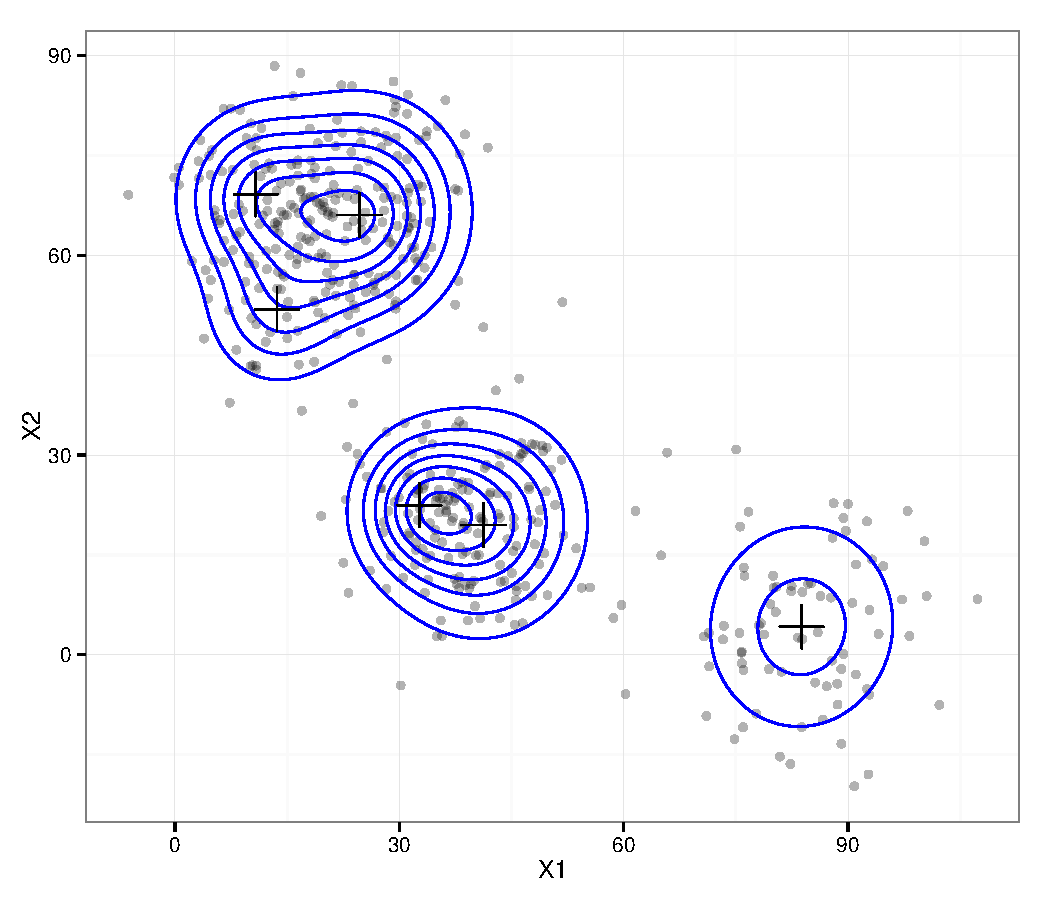
\includegraphics[trim=0cm 0cm 0cm 0cm,width=0.6\textwidth]{partition-example-mixture.pdf} \\
 \end{tabular}
 \caption{Density of a Gaussian mixture with 6 component adjusted to a sample. The Gaussian mean of each component is represented by the symbol `+'. The sample was generated using R \textsc{MixSim} package from a 3 component Gaussian mixture with a max overlapping of $\check{\omega} = 0.01$.}\label{ex_mixture}
\end{center}
\end{figure}

Let $I = \{1,2,3,4,5,6\}$. As commented before, any partition of $I$ yields to a feasible final classification using Eq.\ref{cluster_criteria}. For example, the partition
\[
\mathcal{I}_6 = \{\{1\},\{2\},\{3\},\{4\},\{5\},\{6\}\}
\]
of $I$ yields to a classification where each observation $\m x_i \in \mathbb{R}^2$ is  assigned to the part $\{j\}$ with maximum $\hat{\tau}_{i\{j\}}$. In Figure~\ref{ex_part6} each observation $\m x_i$ is separated according to the assigned part. The isodensity curves for each of the pdf $\hat{f}_{\{j\}} = \phi(\;\cdot\; ; \hat{\m\mu}_j, \hat{\m\Sigma}_j)$, $1\leq j \leq 6$, is included in the graphic.

\begin{figure}[!h]
\begin{center}
\begin{tabular}{cc}
 %   6 toy mixture
  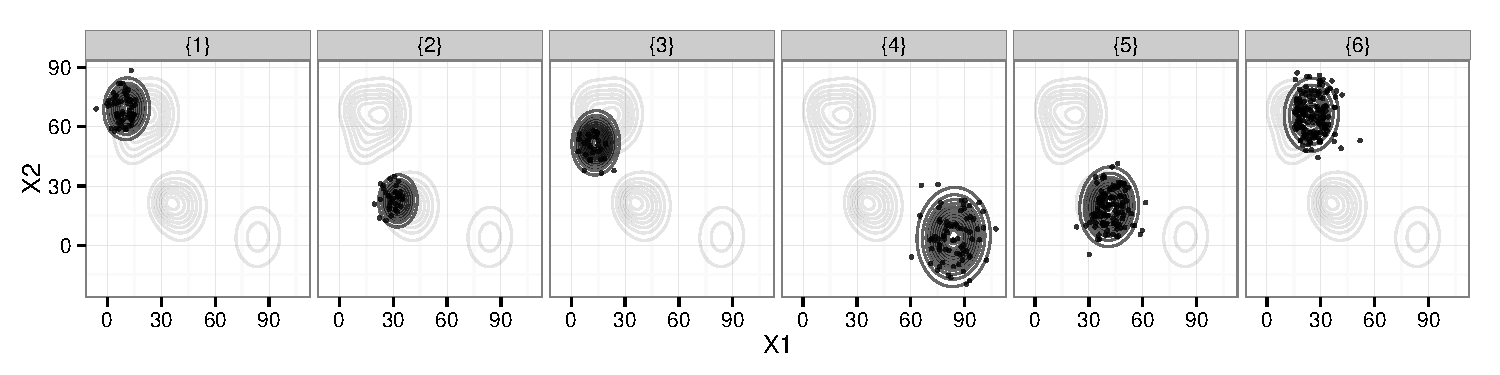
\includegraphics[trim=0cm 0cm 0cm 0cm,width=\textwidth]{partition-example-part6.pdf} \\
 \end{tabular}
 \caption{Classification obtained considering the component partition $\{ \{1\}, \{2\}, \{3\}, \{4\}, \{5\}, \{6\} \}$ with 6 parts in sample $X_{500}$.}\label{ex_part6}
\end{center}
\end{figure}

If we consider a different partition such as
\[\mathcal{I}_3 = \{\{1, 3, 6\},\{2, 5\},\{4\}\}\]
which is grouping those components with closest mean, we get the 3 clusters given in Figure~\ref{ex_part3a}. We have included the isodensity curves of pdf $\hat{f}_{\{1,3,6\}}$, $\hat{f}_{\{2, 5\}}$ and $\hat{f}_{\{4\}}$ given by

\[
%\left\{
\begin{array}{r c l}
\hat{f}_{\{1,3,6\}} & = & \frac{1}{0.52}(0.13 \phi(\;\cdot\; ; \hat{\m\mu}_1, \hat{\m\Sigma}_1) + 0.07 \phi(\;\cdot\; ; \hat{\m\mu}_3, \hat{\m\Sigma}_3) + 0.32 \phi(\;\cdot\; ; \hat{\m\mu}_6, \hat{\m\Sigma}_6)), \\
\hat{f}_{\{2, 5\}} & = &  \frac{1}{0.33}(0.09 \phi(\;\cdot\; ; \hat{\m\mu}_2, \hat{\m\Sigma}_2) + 0.24 \phi(\;\cdot\; ; \hat{\m\mu}_5, \hat{\m\Sigma}_5)), \\
\hat{f}_{\{4\}} & = &\phi(\;\cdot\; ; \hat{\m\mu}_4, \hat{\m\Sigma}_4).
\end{array}
%\right.
\]



\begin{figure}[!h]
\begin{center}
\begin{tabular}{cc}
  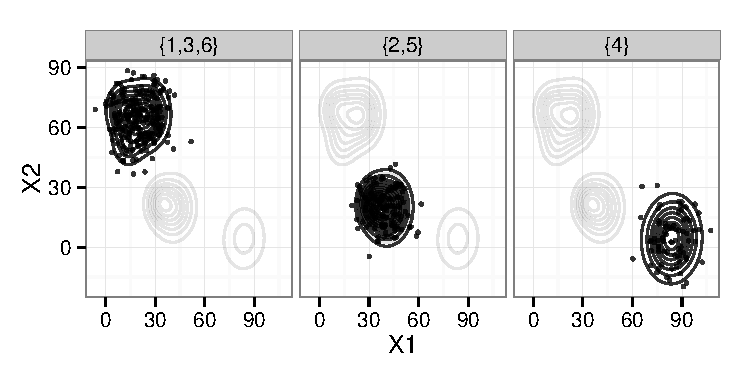
\includegraphics[trim=0cm 0cm 0cm 0cm,width=0.6\textwidth]{partition-example-part3a.pdf} \\
 \end{tabular}
 \caption{Classification obtained considering the component partition $\{\{1, 3, 6 \}, \{2, 5\}, \{5\}\}$ with 3 parts in sample $X_{500}$.}\label{ex_part3a}
\end{center}
\end{figure}

Consider now the hierarchical combination of components given by the following sequence of partitions
\begin{equation}
\begin{array}{r c c}
\mathcal{H}(\mathcal{I}) &=& \{ \{\{1\},\{2\},\{3\},\{4\},\{5\},\{6\}\}, \\
   & & \{\{1, 6\},\{2\},\{3\},\{4\},\{5\} \}, \\
   & &    \{\{1, 6, 3\},\{2\},\{4\},\{5\} \}, \\
   & &    \{\{1, 6, 3\},\{2, 5\},\{4 \} \}, \\
    & &   \{\{1, 6, 3\},\{2, 4, 5\} \}, \\
   & &    \{\{1, 2, 3, 4, 5, 6\}\} \}.
\end{array}
\label{hier_ex}
\end{equation}
Each partition from the hierarchical combination of components given by \ref{hier_ex} defines a clustering where each element is classified to one of the parts of each partition. Therefore, a hierarchical combination of components defines a hierarchical clustering structure. Figure~\ref{hierarchical} shows the hierarchical clustering obtained in sample $X_{500}$ using the hierarchical combination of components given in Eq~\ref{hier_ex}. The first partition $\{\{1\},\{2\},\{3\},\{4\},\{5\},\{6\}\}$ defines a clustering with 6 clusters, the partition $\{\{1, 6\}, \{3\},\{2\},\{4\},\{5\} \}$ defines a clustering with 5 clusters, and so on.

\begin{figure}[thbp]
\begin{center}
\begin{tabular}{cc}
  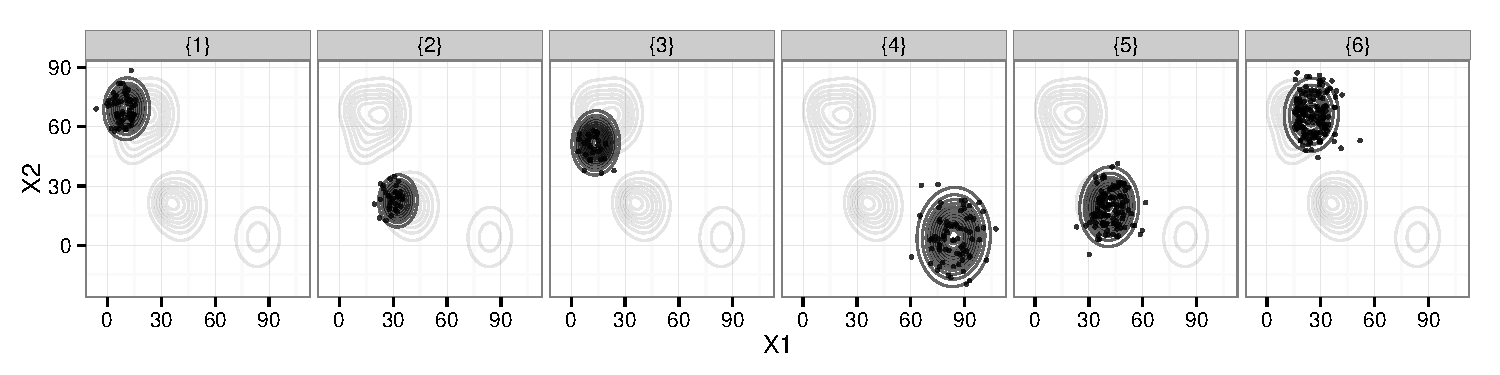
\includegraphics[trim=0cm 0cm 0cm 0cm,width=\textwidth]{partition-example-part6.pdf} \\
    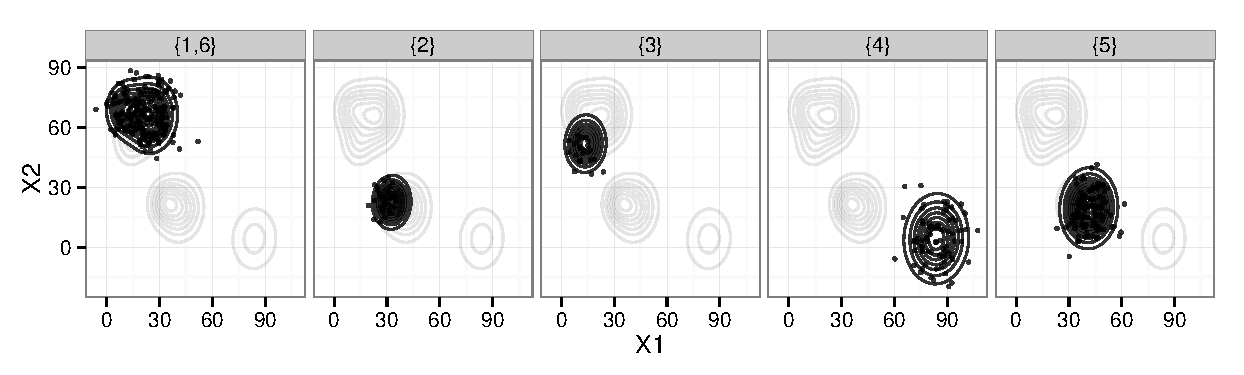
\includegraphics[trim=0cm 0cm 0cm 0cm,width=0.83\textwidth]{partition-example-part5.pdf} \\
      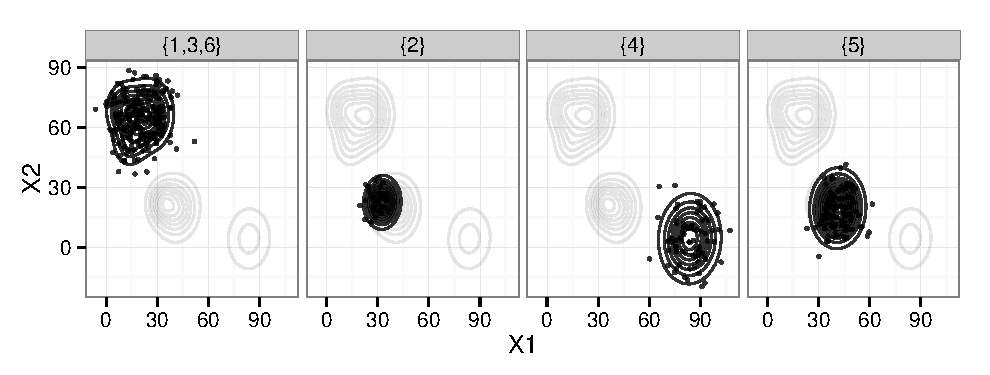
\includegraphics[trim=0cm 0cm 0cm 0cm,width=0.67\textwidth]{partition-example-part4.pdf} \\
        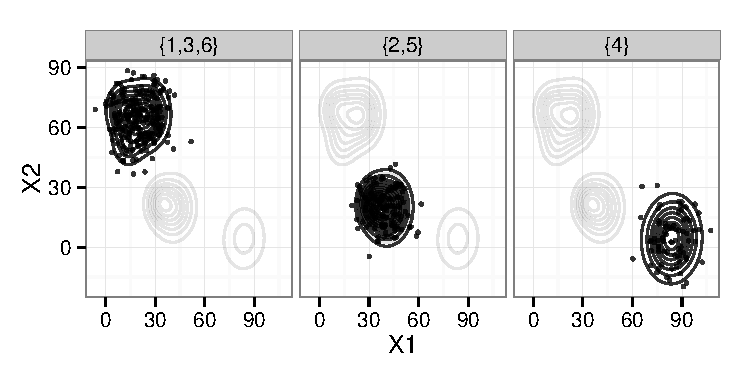
\includegraphics[trim=0cm 0cm 0cm 0cm,width=0.5\textwidth]{partition-example-part3a.pdf} \\
          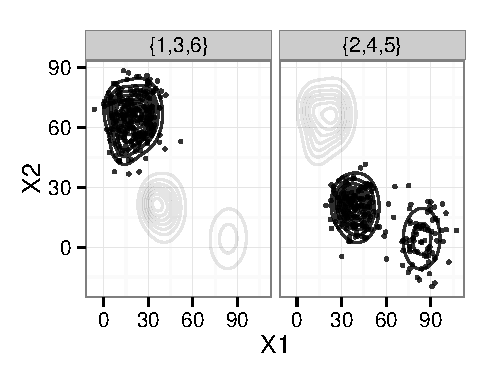
\includegraphics[trim=0cm 0cm 0cm 0cm,width=0.33\textwidth]{partition-example-part2.pdf} \\
            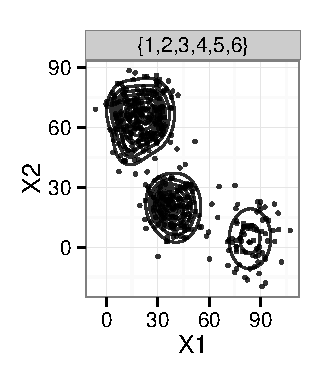
\includegraphics[trim=0cm 0cm 0cm 0cm,width=0.2\textwidth]{partition-example-part1.pdf}
 \end{tabular}
 \caption{Hierarchical cluster obtained by the hierarchical combination of components.}\label{hierarchical}
\end{center}
\end{figure}

In this paper, we review different approaches that we can find in the literature \citep{baudry2010combining, hennig2010methods} to combine the components of a \fmm using the posterior probabilities. Using similar ideas that previous methods, we introduce different new approaches inspired on the geometric nature of the posterior probabilities i.e using the log-ratio approach. Then, we introduce  introduce a generic definition where an integrated formulation unifies all these merging methods.  This formulation opens a way to define new methods based on the posterior probabilities. For example, based on ideas introduced by \cite{longford2014}, we extend the family of methods for merging components using posterior probabilities.  Importantly, although this approaches have been commonly presented for Gaussian mixtures \citep{longford2014,melnykov2013distribution,hennig2010methods,baudry2010combining}, they can be applied using any other probability distribution mixtures because they are based only on the posterior probabilities vectors $\hat{\m\tau}_{i \mathcal{P}_s}$.

The paper is organised as follows: In Section~\ref{old_methods}, the approaches by \cite{hennig2010methods} and \cite{baudry2010combining} to obtain a hierarchical combination of components are presented using the new notation also adopted for the new proposals. This new notation is the crucial element for the integrated formulation that unifies the methods. In Section~\ref{comparison} a comparison of the different approaches is done using simulated data sets. Finally, Section~\ref{conclusions} contains the conclusions and final remarks.


\section{Hierarchical combination of components}
\label{old_methods}


\subsection{Approach based on Shannon entropy}

The Shannon entropy of a posterior probability vector $\hat{\m\tau}_{i \mathcal{P}_s} = \left( \hat{\tau}_{i I_1} , \dots, \hat{\tau}_{i I_s}  \right)$ of an observation $x_i$, $1 \leq i \leq n$ is
\[
Ent( \hat{\m \tau}_{i \mathcal{P}_s} ) = - \sum_{j=1}^s \hat{\tau}_{i I_j}  log(\hat{\tau}_{i I_j} ).
\]
$Ent( \hat{\m \tau}_{i \mathcal{P}_s} )$ is a concave function with its maximum at $(\frac{1}{s},\dots,\frac{1}{s})$. In terms of posterior probabilities, the maximum is obtained when the probability of $\m x_i$ being generated by distribution $\hat{f}_{I_j}$ is the same for $j$, $1\leq j \leq s$. Due to the fact the maximum is the point with more ``confusion'' between parts, \cite{baudry2010combining} proposed to merge those components, $I_a$ and $I_b$, forming a new partition\[ \mathcal{P}_{s-1} = \left( \mathcal{P}_s \setminus \{ I_a, I_b \} \right) \cup \left\{ \in I_a\cup I_b \right\} \] in such a way that $\sum_{i=1}^n Ent( \hat{\m \tau}_{i \mathcal{P}_{s-1}} )$ is maximum. In other words, the criteria proposes to merge those components that after merging, the sum of the entropy of the resulting posterior probability vectors is maximum. The calculation of the previous criteria depends on the posterior probability of each part $\hat{\tau}_{i I_1}, \dots,\hat{\tau}_{i I_s}$. To reduce calculations \cite{baudry2010combining} proposed to combine those parts, $I_a$ and $I_b$, such that the difference
\begin{multline*}
\Delta Ent_{const}(\hat{\m \tau}_{i \mathcal{P}_s}, a, b) = \sum_{i=1}^n Ent( \hat{\m \tau}_{i \mathcal{P}_{s-1}}) - \sum_{i=1}^n Ent( \hat{\m \tau}_{i \mathcal{P}_s}) =  \\ = \sum_{i=1}^n  \left( \hat{\tau}_{i I_{a\cup b}}  log(\hat{\tau}_{i I_{a\cup b}} ) +  \sum_{\substack{j=1 \\
                                                            j \neq a, b}}^s \hat{\tau}_{i I_j}  log(\hat{\tau}_{i I_j} ) \right)  - \sum_{i=1}^n \sum_{j=1}^s \hat{\tau}_{i I_j}  log(\hat{\tau}_{i I_j} ) = \\  =   \sum_{i=1}^n  (\hat{\tau}_{i I_a}+\hat{\tau}_{i I_b}) \log(\hat{\tau}_{iI_a} + \hat{\tau}_{i I_b}) - \sum_{i=1}^n \left\{ \hat{\tau}_{i I_a} \log(\hat{\tau}_{i I_a}) + \hat{\tau}_{iI_b} \log(\hat{\tau}_{i I_b})\right\}
\end{multline*}
is maximum. Importantly, note that this criteria depends only on the posterior probability of $\hat{\tau}_{iI_a}$ and $\hat{\tau}_{iI_b}$. Indeed, once the vectors $\hat{\m\tau}_{i \mathcal{P}_s}$ are calculated for the partition $\mathcal{P}_k$, the hierarchical merging procedure makes the clusters regardless the type of pdf $f_j$ used to fit the \fmm.

\subsection{Directed Estimated Misclassification Probabilities (DEMP) approach}

\cite{hennig2010methods} proposed to combine the two parts $I_a$ and $I_b$ from $ \mathcal{P}_s$ such that \emph{the probability of classifying an observation generated from component $\hat{f}_{I_a}$ to component $\hat{f}_{I_b}$} is maximum. To estimate that probability,  \cite{hennig2010methods} suggested to use a consistent estimator, the Directed Estimated Misclassification Probabilities (DEMP), which can be formulated as
\begin{equation}\label{demp_criteria}
DEMP(\hat{\m \tau}_{i \mathcal{P}_s}, a, b) =\frac{ \sum_{i=1}^n {\hat{\tau}_{i I_a} \mathbbm{1}\left( \forall j\; \hat{\tau}_{i I_{b}} \geq \hat{\tau}_{i I_j} \right)}}{\sum_{i=1}^n \hat{\tau}_{i I_a} },
\end{equation}
where $\mathbbm{1}\left( \cdot \right)$ is the indicator function. Then, \cite{hennig2010methods} proposed to combine parts $I_a$ and $I_b$, such that the $DEMP(\hat{\m \tau}_{i \mathcal{P}_s}, a, b)$ is maximum.

Note that the idea behind the approach proposed by \cite{baudry2010combining} is different from the one proposed by \cite{hennig2010methods}. In the former, the confusion between part $I_a$ and part $I_b$ is measured by measuring how different $\hat{\m \tau}_{i \mathcal{P}_a}$ and $\hat{\m \tau}_{i \mathcal{P}_b}$ are, for all $i$, $1\leq i \leq n$, independently. In contrast, \cite{hennig2010methods} measures the confusion between part $I_a$ and part $I_b$ by counting the number of times an observation is classified to $I_b$, weighing the counting with respect the posterior probability of begin generated by $\hat{f}_{I_a}$ (Eq.~\ref{demp_criteria}).

\subsection{The log-ratio approaches}
\label{lr_approach}

In the total Entropy approach, confusion between components is measured using the notion that the closer the posterior probability vector is from $(\frac{1}{s}, \dots, \frac{1}{s})$ the more confused are the components. Following this notion, we propose to measure the chances of confusing $I_b$ with $I_a$  by measuring how different are $(\frac{\hat{\tau}_{i I_a}}{\hat{\tau}_{i I_a} + \hat{\tau}_{i I_b}}, \frac{\hat{\tau}_{i I_b}}{\hat{\tau}_{i I_a} + \hat{\tau}_{i I_b}})$ from $(\frac{1}{2}, \frac{1}{2})$. That is, we restrict only on the components taking part in the merging process. Moreover, to measure the difference between these two posterior probability vectors, we use the norm defined in the Simplex space. Doing so, we guarantee subcompositional coherence in this measurement \citep{aitchison1986statistical}.The norm of a posterior probability vector, $\| (\hat{\tau}_{iI_a}, \hat{\tau}_{iI_b}) \|$  defined by \cite{aitchison2002simplicial} is \[ \left\| (\hat{\tau}_{iI_a}, \hat{\tau}_{iI_b}) \right\|^2 = \log^2 \left(\frac{ \hat{\tau}_{iI_b} }{ \hat{\tau}_{iI_a} }\right). \] 

In contrast, DEMP approach defines the notion of confusion between two components $I_a$ and $I_b$ by measuring the probability of \emph{classifying an observation to component $I_b$ when the observation was generated from component $I_a$}. Conditioning that the observation is generated by $I_a$ DEMP approach measures this probability by observing if the observation has been classified to $I_b$, i.e.  measuring the value $\mathbbm{1}\left( \forall j\; \hat{\tau}_{i I_{b}} \geq \hat{\tau}_{i I_j} \right)$. Conditioning that the observation is generated by $I_a$ we propose to measure how likely is to classify an observation to $I_b$ when it was generated from $I_a$ by measuring the relative difference between $\hat{\tau}_{i I_b}$ and $\hat{\tau}_{i I_a}$. Therefore, we propose to use the log-ratio between them, i.e.  $\log( \hat{\tau}_{i I_b}/\hat{\tau}_{i I_a})$. Note that, the measure is negative for those observations which are more likely to be assigned to $a$ (to be well classified) and positive for those observation more likely to be assigned to $b$ (to be misclassified). %{\color{blue} Martin: dos comments: \sout{1r. cal posar una frase que com a mínim suggereixi d'on surt la idea de prendre log-ratios.} 2n. no acabo de veure clar que NO calgui agafar valor absolut del logaritme. Quan  les probabilitats són diferents pot molt positiu o molt negatiu i després compensar-se. No sé si no seria millor eliminar-lo directament aquest cas...o posar-lo com a exemple de noves mesures...}

To summarise, using log-ratio approaches we have build two different criteria for measuring the confusion between two parts $(\log ( \hat{\tau}_{iI_b} / \hat{\tau}_{iI_a}) $ and $\log^2 (\hat{\tau}_{iI_b} / \hat{\tau}_{iI_a} ))$. For each of them, we introduce three different strategies to combine the scores obtained for each observation $\m x_i$. This three strategies are
\begin{description}
\item[- const] for each observation, we calculate the confusion measure and we sum (or average) all the confusion measurements.
\item[- prop] for each observation, we calculate the confusion measure and we calculate a weighted mean of them according to the probability of an observation to be generated from component $\hat{f}_{I_a}$.
\item[- dich] for each observation, we calculate the confusion measure and we average the confusions only on those observations associated to component $\hat{f}_{I_a}$.
\end{description}

Table \ref{table_logratio} shows the resulting score functions when the two measures and the three strategies are combined. Measures from first column (log) are based on the confusion measure introduced in DEMP approach. Hence, the measure is not symmetric, in a sense that it is not the same merging $I_a$ to $I_b$ than $I_b$ to $I_a$. By contrast, the confusion for the approaches in the second column are based on the confusion introduced by the Entropy and therefore, it is the same merging $I_a$ to $I_b$ than $I_b$ to $I_a$. Finally, it is important to remark that although the confusion measure (norm) is symmetric, in the case of prop or dich (second and third row) depending on the sample the final measurement it is not symmetric.

%{\color{blue} Martin: potser explicar una mica coses de simetries, de similtuds amb les de Baurdry o Henning o...}

\begin{table}[htpb]
\caption{Log-ratio score functions}
\begin{tabular}{c  c  c c }
 & \multicolumn{1}{c}{} & \multicolumn{1}{c}{}  & \multicolumn{1}{c}{} \\
  & \multicolumn{3}{c}{Measure} \\
\hline
 & \multicolumn{1}{c}{} & \multicolumn{1}{c}{} &  \multicolumn{1}{c}{} \\

 & \multicolumn{1}{c}{} & \multicolumn{1}{c}{log} &  \multicolumn{1}{c}{norm} \\ 
\hline
& const &  $\sum_{i=1}^n \log \left(\frac{ \hat{\tau}_{iI_b} }{ \hat{\tau}_{iI_a} }\right)$ & $ -\sum_{i=1}^n \log^2 \left(\frac{ \hat{\tau}_{iI_b} }{ \hat{\tau}_{iI_a} }\right)$ \\ 

\rotatebox[origin=c]{90}{Scores combination}& prop & $\frac{ \sum_{i=1}^n \hat{\tau}_{iI_a} \log \left(\frac{ \hat{\tau}_{iI_b} }{ \hat{\tau}_{iI_a} }\right)}{\sum_{i=1}^n\hat{\tau}_{iI_a}}$ &   $ \frac{ -\sum_{i=1}^n \hat{\tau}_{iI_a} \log^2 \left(\frac{ \hat{\tau}_{iI_b} }{ \hat{\tau}_{iI_a} }\right)}{\sum_{i=1}^n\hat{\tau}_{iI_a}} $\\ 

& dich & $\frac{ \sum_{i=1}^n  \mathbbm{1}\left( \forall j\; \hat{\tau}_{i I_{a}} \geq \hat{\tau}_{iI_j} \right) \log \left(\frac{ \hat{\tau}_{iI_b} }{ \hat{\tau}_{iI_a} }\right)}{\sum_{i=1}^n \mathbbm{1}\left( \forall j\; \hat{\tau}_{i I_{a}} \geq \hat{\tau}_{iI_j} \right)}$ & $\frac{- \sum_{i=1}^n \mathbbm{1}\left( \forall j\; \hat{\tau}_{i I_{a}} \geq \hat{\tau}_{iI_j} \right) \log^2 \left(\frac{ \hat{\tau}_{iI_b} }{ \hat{\tau}_{iI_a} }\right)}{\sum_{i=1}^n \mathbbm{1}\left( \forall j\; \hat{\tau}_{i I_{a}} \geq \hat{\tau}_{iI_j} \right)} $\\ 


\end{tabular}
\label{table_logratio}
\end{table}





\subsection{Integrated formulation for merging components}
\label{confusion}

Let $\lambda(\hat{\m \tau}_{i \mathcal{P}_s}, a, b)$ be a function measuring the chances of mixing up the mixture component $\hat{f}_{I_a}$ by the mixture component $\hat{f}_{I_b}$ when $\hat{\m \tau}_{i \mathcal{P}_s}$ is known, i.e. selecting $\hat{f}_{I_b}$ when one have to select $\hat{f}_{I_a}$. In Section~\ref{old_methods} we have seen different alternatives to measure such confusion. This alternatives were

\begin{itemize}
\item the entropy presented by \cite{baudry2010combining},
\[\lambda(\hat{\m \tau}_{i \mathcal{P}_s}, a, b) = (\hat{\tau}_{iI_a}+\hat{\tau}_{iI_b}) \log(\hat{\tau}_{iI_a} + \hat{\tau}_{iI_b}) - \hat{\tau}_{iI_a} \log(\hat{\tau}_{iI_a}) + \hat{\tau}_{iI_b} \log(\hat{\tau}_{iI_b}),\]
%\item the misclassification probability presented by \cite{hennig2010methods}, \[\lambda(\hat{\m \tau}_{i \mathcal{P}_s}, a, b) = \mathbbm{1}\left( \forall j\; \hat{\tau}_{i I_{b}} \geq \hat{\tau}_{iI_j} \right),\]
%\item the ``misgeneration'' probability presented by \cite{longford2014}, \[\lambda(\hat{\m \tau}_{i \mathcal{P}_s}, a, b) = \frac{\hat{\tau}_{iI_b}}{\hat{\tau}_{iI_a} + \hat{\tau}_{iI_b}},\]{\color{blue} Marc: Després d'eliminar el mètode DEGP de la secció anterior aquesta mesura és nova pel lector. Millor posar-la quan es presenti el mètode més endavant}
\item the Aitchison norm, \[\lambda(\hat{\m \tau}_{i \mathcal{P}_s}, a, b) = \log^2 (\frac{ \hat{\tau}_{iI_b} }{ \hat{\tau}_{iI_a} }) \text{ and}\]
\item the log-ratio \[ \lambda(\hat{\m \tau}_{i \mathcal{P}_s}, a, b) = \log (\frac{ \hat{\tau}_{iI_b} }{ \hat{\tau}_{iI_a} }).\]
\end{itemize}

All this approaches provide us with different ways to measure the confusion between components. Moreover, all of them are based only on the posterior probability
vector $(\hat{\tau}_{i I_{1}}, \dots, \hat{\tau}_{i I_{s}})$.

Let $\omega(\hat{\m \tau}_{i \mathcal{P}_s}, a)$ be a function measuring the relevance $\hat{\m \tau}_{i \mathcal{P}_s}$ to measure the chances of mixing up  the mixture component $\hat{f}_{I_a}$. In Subsection~\ref{lr_approach} we have seen three different criteria:

\begin{itemize}
\item each observation is equally relevant to measure the chances of mixing up  $\hat{f}_{I_a}$,
\[\omega(\hat{\m \tau}_{i \mathcal{P}_s}, a) = const,\]
\item the relevance is equal to the posterior probability of being generated by  $\hat{f}_{I_a}$,
\[\omega(\hat{\m \tau}_{i \mathcal{P}_s}, a) =  \hat{\tau}_{iI_a} \text{ and}\]
\item  only the posterior probability of observations classified in the part   $I_a$ are relevant
\[\omega(\hat{\m \tau}_{i \mathcal{P}_s}, a) = \mathbbm{1}\left( \forall j\; \hat{\tau}_{i I_{a}} \geq \hat{\tau}_{iI_j} \right).\]
\end{itemize}



For a partition $\mathcal{P}_s = \{ I_1, \dots, I_s\}$ and with  functions $\lambda(\hat{\m \tau}_{i \mathcal{P}_s}, a, b)$ and $\omega(\hat{\m \tau}_{i \mathcal{P}_s}, a)$ fixed, we can define a mixture component merging approach as follows: if $\hat{\m\tau}_{i \mathcal{P}_s} = \left( \hat{\tau}_{i I_1} , \dots, \hat{\tau}_{i I_s}  \right)$ is the posterior probability vectors of observation $x_i$, $1 \leq i \leq n$,  merge those two parts $I_a$ and $I_b$, into one part $I_a \cup I_b$ which maximise
\begin{equation}\label{unifying_equation}
S_{\omega, \lambda}( \hat{\m \tau}_{i \mathcal{P}_s}, a, b) = \frac{\sum_{i=1}^n \omega(\hat{\tau}_{i \mathcal{P}_s}, I_a) \lambda(\hat{\tau}_{i \mathcal{P}_s}, I_a, I_b)}{\sum_{i=1}^n \omega(\hat{\tau}_{i \mathcal{P}_s}, I_a) }.
\end{equation}


The general confusion measure given by Equation~\ref{unifying_equation} contains all the approaches introduced in Section~\ref{old_methods}. Note that when $\omega(\hat{\tau}_{i \mathcal{P}_s}, I_a) = const$ maximising Equation~\ref{unifying_equation} is equivalent to maximise
\[
S_{\omega, \lambda}( \hat{\m \tau}_{i \mathcal{P}_s}, a, b) = \sum_{i=1}^n \lambda(\hat{\tau}_{i \mathcal{P}_s}, I_a, I_b)
\]
and therefore, Equation~\ref{unifying_equation} also includes as particular cases the Entropy approach, const-log and const-norm approaches. Particularly, by using the functions $\lambda(\hat{\m \tau}_{i \mathcal{P}_s}, a, b)$ and $\omega(\hat{\m \tau}_{i \mathcal{P}_s}, a)$ already defined in Section~\ref{old_methods} we have all the combinations given by Table~\ref{table_methods}. Note that the method with $\lambda(\hat{\m \tau}_{i \mathcal{P}_s}, a, b) =  \mathlarger{\mathbbm{1}}\left\{  \forall \ell \; \tau_{hb} \geq \tau_{h\ell}  \right\}$ and  $\omega(\hat{\m \tau}_{i \mathcal{P}_s}, a) = \mathlarger{\mathbbm{1}}\left\{  \forall \ell\; \; \tau_{ia} \geq \tau_{i\ell}  \right\}$ it always evaluate 0, and therefore, it is of no use.

A part of containing the approaches from Section~\ref{old_methods}, Equation~\ref{unifying_equation} permits to introduce a broad range of new approaches by varying functions $\lambda(\hat{\m \tau}_{i \mathcal{P}_s}, a, b)$ and $\omega(\hat{\m \tau}_{i \mathcal{P}_s}, a)$. For example, \cite{longford2014} proposed to measure the confusion between two component $I_a$ and $I_b$ by measuring the probability of $\m x_i$ being generated by $\hat{f}_{I_b}$ conditioned to $\m x_i$  being generated by $\hat{f}_{I_a}$ or $\hat{f}_{I_b}$. In other words, they proposed to measure the confusion between components by measuring $\frac{\hat{\tau}_{iI_b}}{\hat{\tau}_{iI_a} + \hat{\tau}_{iI_b}}$. Although the approach presented in \cite{longford2014} was estimated by simulation. In this paper, one can use their notion of confusion defining
\[\lambda(\hat{\m \tau}_{i \mathcal{P}_s}, a, b) = \frac{\hat{\tau}_{iI_b}}{\hat{\tau}_{iI_a} + \hat{\tau}_{iI_b}}.\]
Combining with the already defined weighing functions, we get three new methods to combine components. 

The notion of confusion given by DEMP criteria is similar to the one given at \cite{longford2014}. The former estimates the probability of \emph{classifying} an observation $\m x_i$ to $I_b$ when the observation was generated by $I_a$, whereas the later estimates the probability of $\m x_i$ being \emph{generated} by $\hat{f}_{I_b}$ conditioned to $\m x_i$  being generated by $\hat{f}_{I_a}$ or $\hat{f}_{I_b}$. Because of this, we refer to the methods derived from \cite{longford2014} by Directed Estimated Generation Probabilities methods (DEGP). Note that the main difference between the approach proposed in \cite{longford2014} and the ones introduced here are that the first is an estimator obtained by simulation, the second is obtained directly from sample $\m X$.

\begin{table}[htpb]
\caption{Different combinations of score functions}
\begin{tabular}{c  c | >{\centering}m{0.7in} | >{\centering}m{0.8in} | >{\centering}m{0.7in} | m{0in}}
 & \multicolumn{1}{c}{} & \multicolumn{1}{c}{} & \multicolumn{1}{c}{} & \multicolumn{1}{c}{} & \multicolumn{1}{c}{}\\
 & \multicolumn{1}{c}{} & \multicolumn{3}{c}{$\omega(\boldsymbol\tau_i, a)$} &\\

 & \multicolumn{1}{c}{} & \multicolumn{1}{c}{} & \multicolumn{1}{c}{} & \multicolumn{1}{c}{} & \multicolumn{1}{c}{}\\

 & \multicolumn{1}{c}{} & \multicolumn{1}{c}{1} & \multicolumn{1}{c}{$\tau_{ia}$} & \multicolumn{1}{c}{$\mathlarger{\mathbbm{1}}\left\{ \forall \ell\;\tau_{ia}\geq \tau_{i\ell}  \right\}$} &\\ \cline{3-5}

& $\large\substack{(\tau_{i a}+\tau_{i b}) \log(\tau_{i a} + \tau_{i b}) - \\ - \tau_{i a} \log(\tau_{i a}) - \tau_{i b} \log(\tau_{i b}) }$ & {\small const-entr}\\($\Delta Ent$)& {\small prop-entr} & {\small dich-entr } &\\[5em] \cline{3-5}

& $\mathlarger{\mathbbm{1}}\left\{  \forall \ell \; \tau_{hb} \geq \tau_{h\ell}  \right\}$ & {\small const-demp} & {\small prop-demp}\\($DEMP$)  & {\small dich-demp} & \\[5em] \cline{3-5}

\rotatebox[origin=c]{90}{$\lambda(\boldsymbol\tau_i, a, b)$}& ${\tau_{i b}}({\tau_{i a}+\tau_{i b}})^{-1}$ & {\small const-degp} &  {\small prop-degp}  & {\small dich-degp} &\\[5em] \cline{3-5}

& $\log{\tau_{i b} / \tau_{i a}}$ & {\small const-log} & {\small prop-log}  & {\small dich-log}  &\\[5em] \cline{3-5}

& $\log^2{\tau_{i b} / \tau_{i a}}$ & {\small const-norm}  & {\small prop-norm} & {\small dich-norm}   &\\[5em] \cline{3-5}
\end{tabular}
\label{table_methods}
\end{table}

In Table~\ref{table_methods} we summarise the methods presented in this Section in introduce a name to refer to. In parenthesis we denote the methods introduced by \cite{baudry2010combining} and \cite{hennig2010methods}. In next Section we analyse the main differences between them.

\section{Evaluating the performance of the methods}
\label{comparison}

\subsection{A simple example with fixed parameters}

%{\color{blue} Martin: a partir d'aquí no he tocat res, tinc comentaris petits com: 1. per què ara les f porten barret?; 2. canviar la lletra w del overlaping level per theta o similar, es confon amb la funció w dels apartats anteriors. També tinc un comentari més important: en aquest apartat del simple case jo deixaria o bé la mixtura de 2 o bé la mixtura de 3, però no les dues. Agafa la més informativa (la de 2?) i l'altra la resumeixes dient que si es fes es veuria fàcilement que aleshores surt una altra cosa...no sé si m'explico..}

In this section we consider a very simple example to compare the confusion measure given by each method from Table~\ref{table_methods}.


Consider the \fmm
\begin{equation}\label{two_mixture}
f_2 = \pi_a f_{I_a} + (1 - \pi_a) f_{I_b, \mu_b}
\end{equation}
with \emph{two} components, where component $f_{I_a} = N(0, 1)$ is the univariate normal distribution with mean equal to $0$ and variance $1$, and component $\hat{f}_{I_b, \mu_b} = N(\mu_b, 1)$ is a normal distribution with mean $\mu_b$ and variance $1$, and the two mixture proportions are parameterised by $\pi_a$. We study Equation~\ref{unifying_equation} with respect to mixture $f_2$ when parameters $\pi_a$ and $\mu_b$ change. 

For a fixed $\pi_a$ and $\mu_b$ we generate a sample $\m X$ of size $n=500$ randomly generated from mixture $f_2$. For each element $x_i$ of $\m X$, we calculate the posterior probability vector $\hat{\m \tau}_{i \{\{a\},\{b\}\}}$. To reduce variation in the final estimates, instead of adjusting a finite mixture distribution to  sample $\m X$, we have assumed $\hat{f}{I_a} = f_{I_a}$ and $\hat{f}{I_b} = f_{I_b}$. Then, for each approach presented in this paper (see  Table~\ref{table_methods}), we calculate the confusion between $f_{I_a}$ and $f_{I_b}$ using Equation~\ref{unifying_equation}. We have repeated the process $100\;000$ times and averaged the confusion measured by each approach. Figure~\ref{fig:mu_varying} summarises the results obtained.

\begin{figure}[!t]
\centering
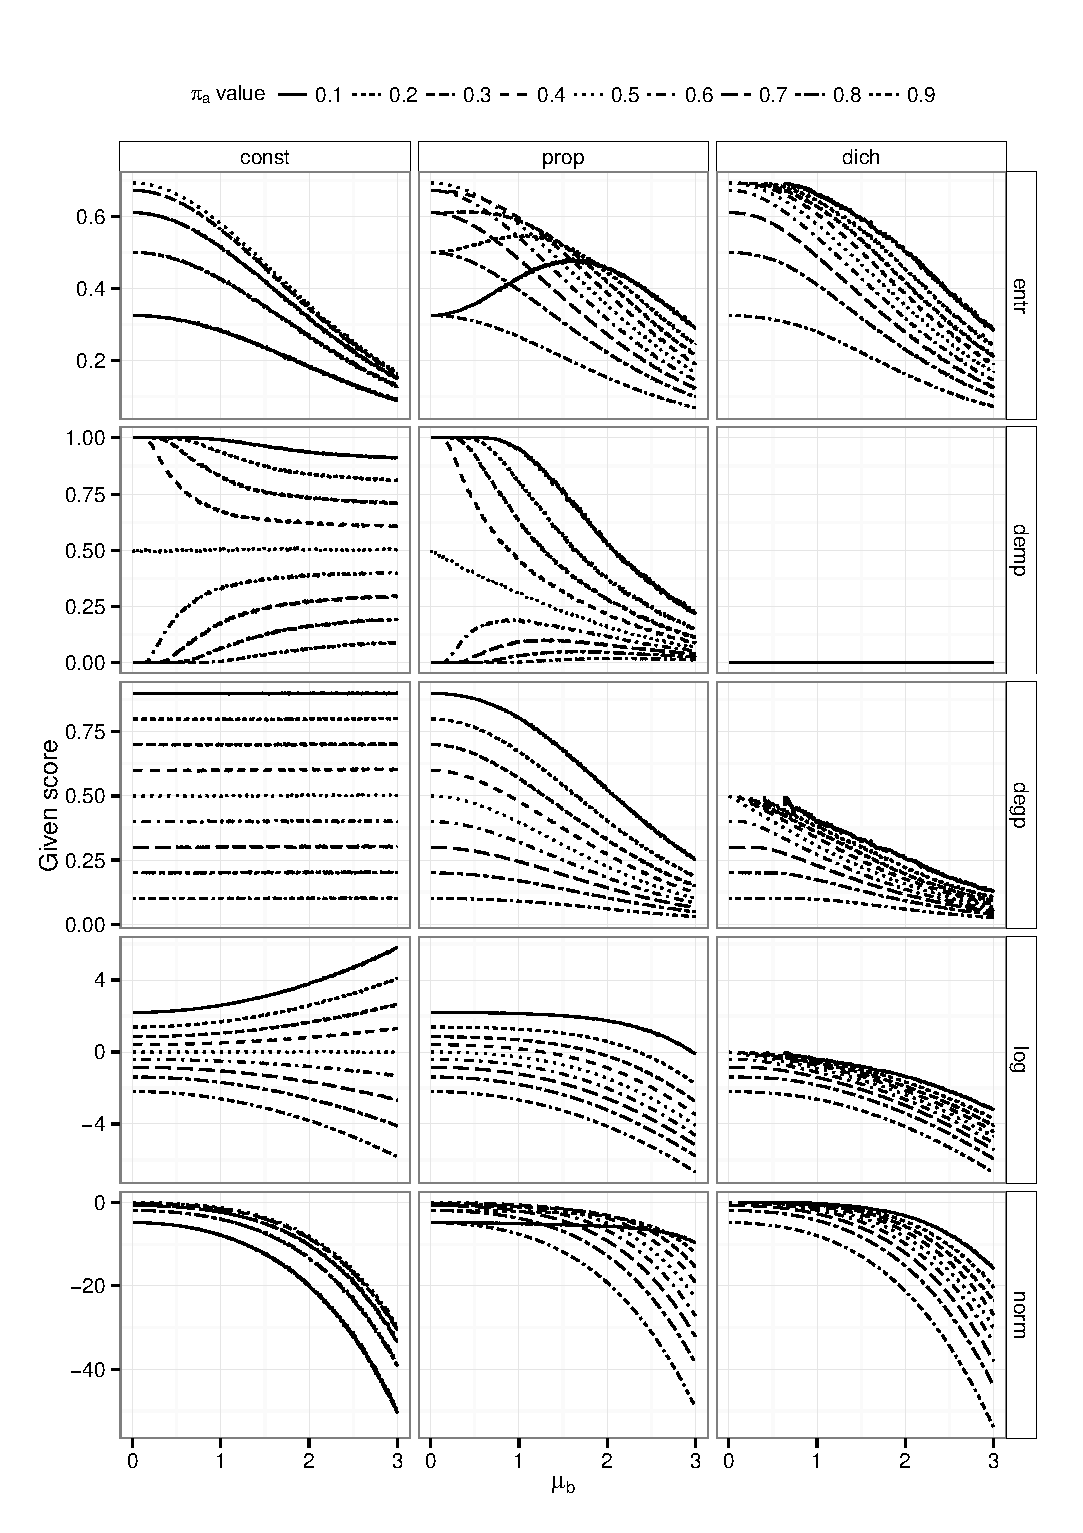
\includegraphics[scale=.5]{fig01all.eps}
\caption{Confusion measurement averaged over 100\;000 simulations for different functions $\lambda$ and $\omega$ varying $\mu_b$ from 0 to 1 and $\pi_a \in \{0.1, 0.2, 0.3, 0.4, 0.5, 0.6, 0.7, 0.8, 0.9\}$ }
\label{fig:mu_varying}
\end{figure}

In the first column methods with $\omega(\hat{\m \tau}_{i \mathcal{P}_s}, a) = 1$ are shown. In this scenario, with respect $\mu_b$ only the entropy approach (const-entr) and the norm approach (const-norm) perform as expected, that is, the confusion between $I_a$ and $I_b$ decreases as the distance between the centre of distribution $\hat{f}_{I_a}$ and $\hat{f}_{I_b, \mu_b}$ increase. const-degp approach, in contrast to const-demp and const-log, don't increase as $\mu_b$ increase. With respect $\pi_a$, all methods except the const-entr and const-norm reduce the confusion between $I_a$ and $I_b$ when $\pi_a$ decrease. This is because const-demp, const-degp and const-log are measuring the chances of confusing $I_a$ by $I_b$ (to choose $I_b$ when one has to choose $I_a$). For the const-entr and the const-norm  approaches the confusion is the same when $\pi_a = 1- \pi_a$ and therefore, in the plot the respective lines overlap.



In the second column methods with $\omega(\hat{\m \tau}_{i \mathcal{P}_s}, a) = \hat{\tau}_{iI_a}$ are shown. In this case, with respect $\mu_b$ all the methods perform as expected, the score decreases when $\mu_b$ increases. With respect $\pi_a$, the methods have similar behaviour when $\mu_b$ increases and when $\mu_b$ is close to $0$ the confusion measurement is similar to the confusion using $\omega(\hat{\m \tau}_{i \mathcal{P}_s}, a) = 1$ (first column).

In the third column, the confusion is represented weighing with function $\omega(\hat{\m \tau}_{i \mathcal{P}_s}, a) = \mathbbm{1}\left( \forall j\; \hat{\tau}_{i I_{a}} \geq \hat{\tau}_{iI_j} \right)$. In this case, when  $\lambda(\hat{\m \tau}_{i \mathcal{P}_s}, a, b) = \mathbbm{1}\left( \forall j\; \hat{\tau}_{i I_{b}} \geq \hat{\tau}_{iI_j} \right)$ (dich-demp), the confusion is constantly $0$ and therefore, dich-demp is of no use to decide which components needs to be merged. The other approaches become similar with respect to $\pi_a$ and $\mu_b$.


%To compare, now we include another component keeping the two previous components inside the mixture. Consider the \fmm
%\begin{equation}\label{three_mixture}
%f_3 = \pi_a \hat{f}_{I_a} + (0.5 - \pi_a) \hat{f}_{I_b, \mu_b} + 0.5 \hat{f}_{I_c}
%\end{equation}
%with three components. Component $\hat{f}_{I_a} = N(0, 1)$ is the normal with mean equal to $0$ and variance $1$, component $\hat{f}_{I_b, \mu_b} = N(\mu_b, 1)$ is a normal with mean $\mu_b$ and component $\hat{f}_{I_c} = N(3, 1)$ is the normal with mean equal to $3$ and variance $1$. The two first mixture proportions are parameterised by $\pi_a$ whereas the third one is constantly $0.5$.
%
%Similar to the previous simulation, we have  randomly generated $m=100\;000$ different samples of size $n=500$ from mixture $f_3$. We have evaluated each approach proposed in Table~\ref{table_methods} by varying parameter $\pi_a$ between values $0.05, 0.1, \dots, 0.45$ and parameter $\mu_b$ varying between $0$ and $3$. For each approach and parameter value, we have calculated the mean of the score obtained in each of the $m$ samples. In Figure~\ref{fig:mu_varying3} the obtained means are represented.
%
%\begin{figure}[!t]
%\centering
%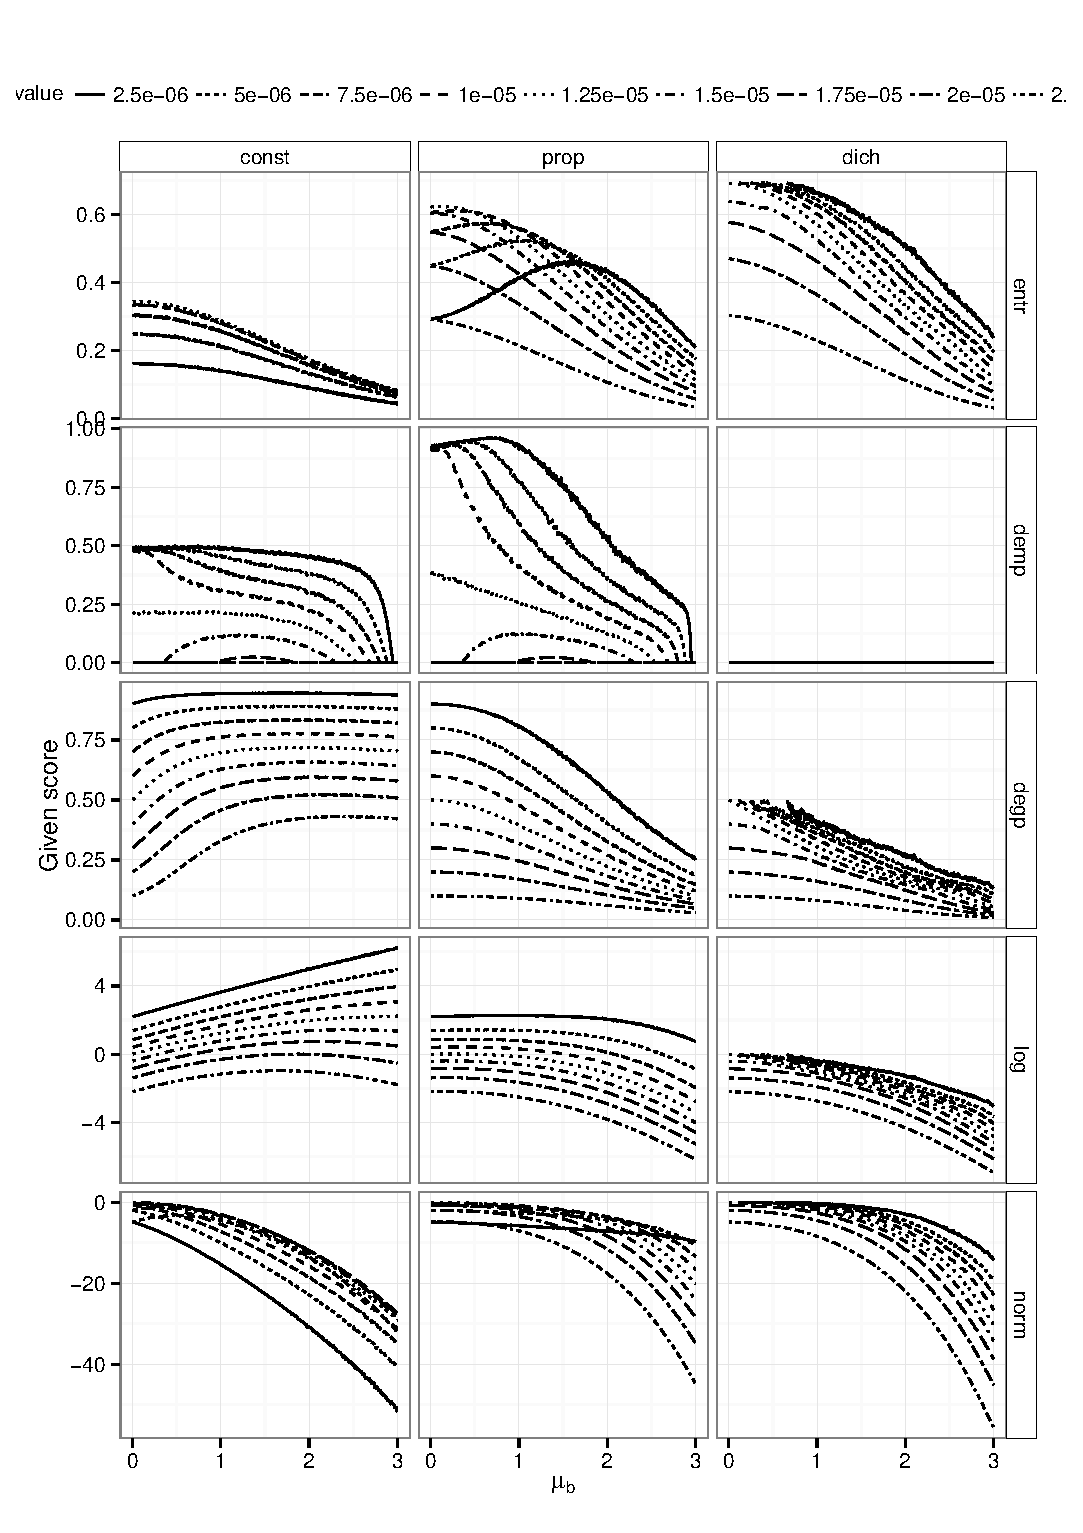
\includegraphics[scale=.5]{fig01ball.eps}
%\caption{Score calculated for methods described for different approaches of $\lambda$ and $\omega$ score when $\mu_b$ varying}
%\label{fig:mu_varying3}
%\end{figure}
%
%
%Now, the main difference between the results obtained in Figure~\ref{fig:mu_varying} and Figure~\ref{fig:mu_varying3} appear on the first column, which corresponds to those methods with the constant weighing function, i.e. $\omega(\hat{\m \tau}_{i \mathcal{P}_s}, a) = const$. {\color{blue} Alguna explicaci\'{o} de perqu\`{e} passa aix\`{o}?}
%
%In each simulation, the second and third column scores the confusion between components similarly. Note that by construction, when the confusion between part $I_a$ and part $I_b$ is calculated with function $\lambda(\hat{\m \tau}_{i \mathcal{P}_s}, a, b)$, methods $DEGP$, $LOG$ and $LOG^2$ score the same whenever the ratio $\frac{\pi_a}{(1 - \pi_a)}$ and $\frac{\pi_a}{(0.5 - \pi_a)}$ is the same for mixture $f_2$ and $f_3$ respectively.


\subsection{Simulation example}

In this section we generate different samples to test the performance of methods available at Table~\ref{table_methods}. To simulate our data sets we use the R package MixSim~\citep{melnikov2012mixsim}. This package permits to generate mixtures with a fixed overlapping level, $\check{\omega}$. The overlapping level $\check{\omega}$ is a measure of how easy is to confuse two components. $\check{\omega}$ is a probability and therefore it ranges between $0$ and $1$. Figure~\ref{ex_mixture} was generated with $\check{\omega} = 0.01$. To compare, in Figure~\ref{omega} three different random samples with $\check{\omega}=0.05$, $\check{\omega}=0.25$ and $\check{\omega}=0.45$ are shown. 

\begin{figure}[!t]
\centering
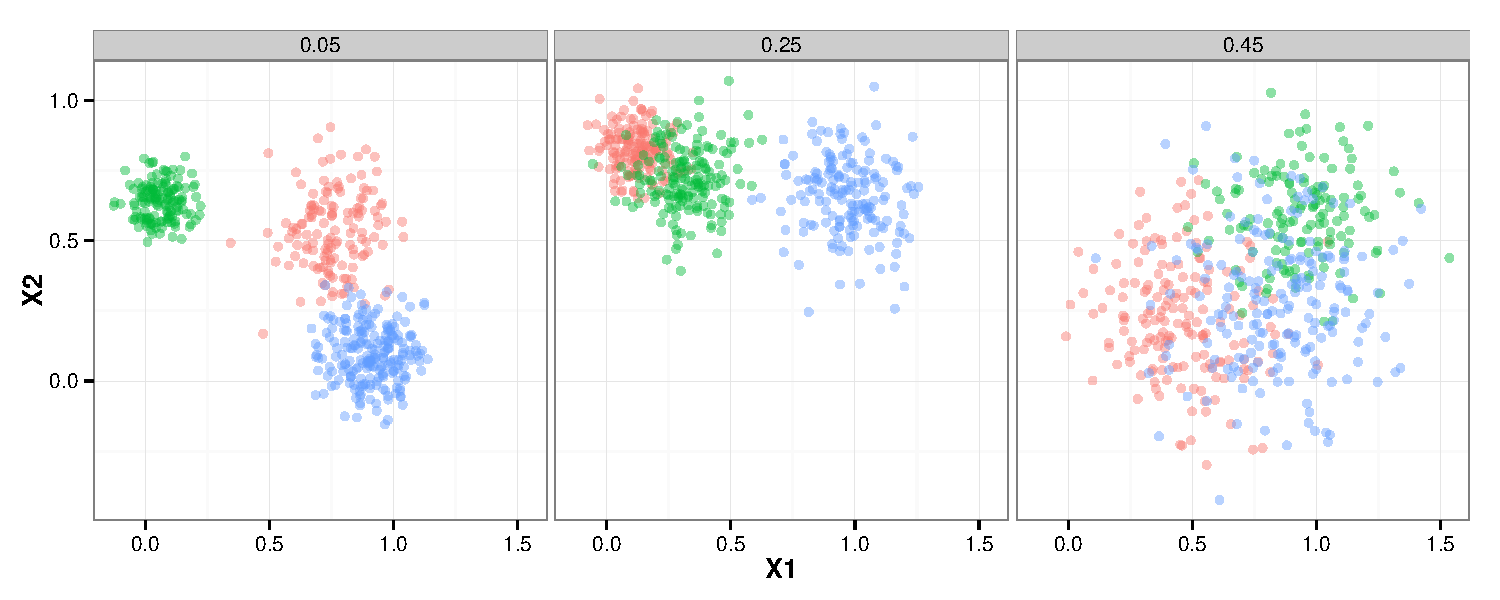
\includegraphics[scale=.5]{omega.pdf}
\caption{Example for different values of parameter $\check{\omega}$}
\label{omega}
\end{figure}


To test the components, we proceed as follow. First, a random sample $\m X$ was generated following a finite mixture with 3 components, we keep the components originating each observation, we consider this the \emph{original cluster}. Then, a finite mixture with 9 components was adjusted to sample $\m X$. We proceed with a merging method until reaching a partition with three elements. Finally, we compared the cluster obtained with the partition with three parts and the original cluster. To compare we use different measures: rand index, the adjusted Rand index, Fowlkes and Mallows index, Mirkin metric variation of information and agreement proportion \citep{meila2006comparing}. Because the final results were similar using each method of comparison, in this article we decide to only report the agreement proportion.

The simulation had the following steps, for different values of $\check{\omega}$ from $0$ to $0.5$ and each method $\mathcal{M}$ from Table~\ref{table_methods},  we repeated $1\,000$ times the following process:
\begin{enumerate}
\item We generated a sample $X$ of size $n=500$ with $D=5$ coordinates coming from a gaussian mixture with $3$ components whose components have maximum overlapping $\check{\omega}$. We kept the component originating each element of sample $X$. Therefore, we had an original partition to which compare.
\item We fitted a mixture with 9 components to sample $X$.
\item Using method $\mathcal{M}$ we built a hierarchical partition as the one shown in Figure~\ref{hierarchical}.
\item We compared the original partition with the 3 element partition obtained with method $\mathcal{M}$. To compare the similarity between the original we used the agreement proportion. The Agreement proportion varies between $0$ and $1$, being $1$ a perfect agreement.
\end{enumerate}

Finally, we averaged for each method $\mathcal{M}$ the agreement proportion obtained over the $1\,000$ simulations.  To compare the performance of each method $\mathcal{M}$, we included a random method which at step $3$  randomly decides the two components to merge. 

\begin{figure}[!h]
\centering
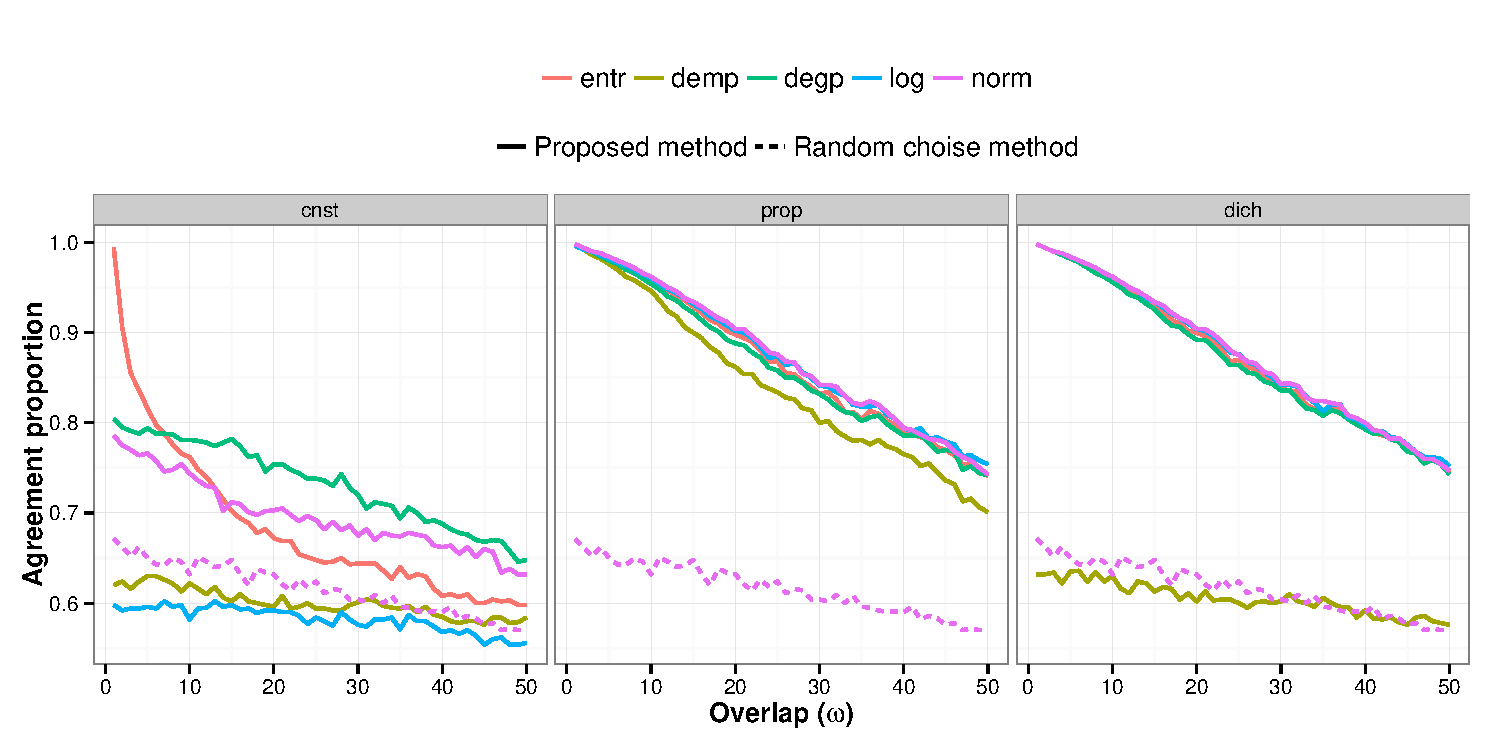
\includegraphics[width=\textwidth]{linesagreement.pdf}
\caption{$\lambda$ Agreement proportion results.}
\label{fig:mub}
\end{figure}

In Figure~\ref{fig:mub} we plot the obtained results. We have separated the methods depending on the weighing function.

In Figure~\ref{fig:mub} left, the methods which use the constant weighing function $\omega(\hat{\m \tau}_{i \mathcal{P}_s}, a) = const$ are represented. For lower levels of overlapping, the Entropy method (cont-entr) (\cite{baudry2010combining}) is the one performing better. For higher level of overlapping, the const-norm and const-demp methods perform slightly better than the others. %This is coherent with the graphics shown in Figure~\ref{fig:mu_varying} where those two methods were the only methods (with constant weighing) decreasing as the distance between distributions increased.

In Figure~\ref{fig:mub} center, the methods weighing the score by the posterior probability of begin generated by component $\hat{f}_{I_a}$, $\omega(\hat{\m \tau}_{i \mathcal{P}_s}, a) =  \hat{\tau}_{iI_a}$, are shown. In this case, all methods perform better than the ones with constant weighing. Between them, the ones with higher agreement proportion were prop-log and prop-norm performing almost equally, the one with lower agreement proportion was prop-demp \citep{hennig2010methods}.

Finally, in Figure~\ref{fig:mub} right, the methods with dichotomic weighing function are shown. The variation for those methods is minimum. Remember that, in this case, the dich-demp method is of no use. At first glance, when using the dichotomic weighing function, the confusion function $\lambda(\hat{\m \tau}_{i \mathcal{P}_s}, a)$ is not very relevant.

\section{Conclusions}
\label{conclusions}

In this paper we have reviewed two different approaches to merge the components of a finite mixture introduced by \cite{hennig2010methods} and \cite{baudry2010combining}. This two methods have in common that to combine the components they only use the information contained on the posterior probabilities. This property allows them to be applied with \fmm base on any family of distributions (Gaussian, Poisson, etc). Based on those two methods, we have presented different methods performing particular well in al the scenarios we have tried. We detected that all the existing methods were sensible to be expressed with a unique formulation. Using this new formulation we were be able to incorporate a new approach using the notion of confusion presented in \cite{longford2014}. 

Finally, we have briefly analysed the methods with respect to some mixture parameters and with respect to the capacity to identify clusters defined from a \fmm. The results suggest that to merge components it is important to weight the confusion $\lambda(\hat{\m \tau}_{i \mathcal{P}_s}, a)$ with respect the relevance of each observation to the specific merging. We have introduced three weighing functions $\omega(\hat{\m \tau}_{i \mathcal{P}_s}, a) = const$ (const), $\omega(\hat{\m \tau}_{i \mathcal{P}_s}, a) = \hat{\tau}_{iI_a}$ (prop) and $\omega(\hat{\m \tau}_{i \mathcal{P}_s}, a) = \mathbbm{1}\left( \forall j\; \hat{\tau}_{i I_{a}} \geq \hat{\tau}_{iI_j} \right)$ (dich), and we have seen that when the const weighing was performing worse in almost all the scenarios.


\bibliographystyle{apalike}
\begin{thebibliography}{}

\bibitem[Aitchison, 1986]{aitchison1986statistical}
Aitchison, J. (1986).
\newblock {\em {The Statistical Analysis of Compositional Data}}.
\newblock Monographs on Statistics and Applied Probability. Chapman \& Hall
  Ltd., London (UK).

\bibitem[Aitchison, 2002]{aitchison2002simplicial}
Aitchison, J. (2002).
\newblock {\em {Simplicial inference}}.
\newblock {\em Algebraic Methods in Statistics anb Probability}, 287: 1--22.

\bibitem[Baudry et~al., 2010]{baudry2010combining}
Baudry, J.-P., Raftery, A.~E., Celeux, G., Lo, K., and Gottardo, R. (2010).
\newblock {Combining Mixture Components for Clustering}.

\bibitem[Hennig, 2010]{hennig2010methods}
Hennig, C. (2010).
\newblock {Methods for merging Gaussian mixture components}.
\newblock {\em Advances in Data Analysis and Classification}, 4(1):3--34.

\bibitem[Lee and Cho, 2004]{lee2004combining}
Lee, H.-j. and Cho, S. (2004).
\newblock {Combining Gaussian Mixture Models}.
\newblock In Yang, Z., Yin, H., and Everson, R., editors, {\em Intelligent Data
  Engineering and Automated Learning – IDEAL 2004 SE - 98}, volume 3177 of
  {\em Lecture Notes in Computer Science}, pages 666--671. Springer Berlin
  Heidelberg.

\bibitem[Longford and Bartosova, 2014]{longford2014}
Longford, N.~T. and Bartosova, J. (2014).
\newblock {A confusion index for measuring separation and clustering}.
\newblock {\em Statistical Modelling}, 14(3):229--255.

\bibitem[Meila, 2006]{meila2006comparing}
Meila, M (2006).
\newblock {Comparing clusterings - an information based distance}.
\newblock {\em Journal of Multivariate Analysis}, 98:873--895.

\bibitem[Melnykov, 2013]{melnykov2013distribution}
Melnykov, V. (2013).
\newblock {On the Distribution of Posterior Probabilities in Finite Mixture
  Models with Application in Clustering}.
\newblock {\em Journal of Multivariate Analysis}, 122:175--189.

\bibitem[Pastore and Tonellato, 2013]{pastore2013merging}
Pastore, A. and Tonellato, S.~F. (2013).
\newblock {A Merging Algorithm for Gaussian Mixture Components}.
\newblock {\em SSRN Electronic Journal}, (04).

\bibitem[Melnykov et~al., 2012]{melnikov2012mixsim}
Melnykov, V. and Chen, W.C. and Maitra, R. (2012).
\newblock {MixSim: An R Package for Simulating Data to Study Performance of Clustering Algorithms}.
\newblock {\em Journal of Statistical Software}, 51(12).

\end{thebibliography}

\end{spacing}

\end{document}
